\documentclass[10pt]{revtex4-1}

\RequirePackage{ifpdf}  % flag for pdf or dvi backend
\ifpdf
  \usepackage[pdftex]{graphicx}
\else
  \usepackage[dvips]{graphicx}
  \usepackage[colorlinks=false,dvips]{hyperref}
\fi
%\DeclareGraphicsRule{.jpg}{eps}{.jpg}{`convert #1 eps:-}

\usepackage{ae}
\usepackage[ngerman, english]{babel}

%\usepackage{SIunits}
%\newcommand\elementarycharge{\textrm{e}}
%\newcommand\mbar{\milli\textrm{bar}}

\usepackage{svg}


\usepackage{amsmath}
\usepackage{amssymb}
\usepackage{setspace}



\renewcommand*{\doi}[1]{\href{http://dx.doi.org/\detokenize{#1}}{doi: \detokenize{#1}}}

\renewcommand*{\tensor}[1]{\hat{#1}}

\renewcommand\r{r}
\newcommand\rmax{r_{max}}
\newcommand\rnorm{r_{n}}

\begin{document}
\pagenumbering{arabic}

\title{Forbes, O Forbes, how shall we understand thee ?}

\author{}
\email{}
\affiliation{}

\date{\today}



\maketitle
\pagestyle{headings}



\section{Nomenclature}

\begin{tabular}{l|l|l}
    My variable name 								& name in Forbes publications & description \\
		$z$ 														& $z,f$												& surface sag \\
		$\r$														& $\rho$											& radial coordinate, distance from optical axis, $\sqrt{x^2+y^2}$ \\
		$\rmax$													& $\rho_{max}$								& clear aperture radius \\
		$\rnorm = \r / \rmax$						& $u = \rho / \rho_{max}$			& normalized radial coordinate \\
		$\xi = \rnorm^2$								& $x = u^2$ 									& \\
		$c$ 														& $c$													& surface curvature (inverse radius) \\
		$\kappa$												& $\epsilon = 1 + \kappa$			& conic constant $\kappa$, excentricity $\epsilon$ \\
		$D$															& $g,D$												& sag Deviation from sphere
\end{tabular}		

\section{Classical Polynomial Aspheres}

Classically, Aspheres are described by
\begin{eqnarray}
	z(\r) &=& \frac{c \r^2}{1+\sqrt{1-(1+\kappa)c^2 \r^2}} + \sum_{m=0}^M b_m \r^m
\end{eqnarray}
While the monomials $\r^m$ are linear independent, they are not orthogonal. When changing one parameter $b_m$, all other parameters have to be reoptimized to compensate possible shoot-offs of the polynomial terms at the border of the asphere. This slows down convergence and bears numerical difficulties in properly conditioning optimization of an optical design. According to Forbes [Forbes 2007], numerical problems arise with double-precision float calculations when dealing with orders $M > 10$.

Therefore, an orthogonal basis is desired. Forbes proposes two different scalar products defining orthogonality and leading to different sets of polynomials: strong and mild Forbes polynomials. [Forbes 2007]

\section{Strong Forbes Aspheres}

\subsection{Introducing the Scalar Product}

\begin{eqnarray}
	z(\r) &=& \frac{c \r^2}{1+\sqrt{1-(1+\kappa)c^2 \r^2}} + D_{strong}(\rnorm)
\end{eqnarray}
The strong Forbes asphere $D_{strong}$ defines the deviation of surface sag from a conic. We introduce a set of basis functions $Q_m$ to describe our asphere.
We use the ansatz
\begin{eqnarray}
	D_{strong}(\rnorm) &=& \sum_{m=0}^M a_m \rnorm^4 Q_m(\rnorm^2) \\
	D_{strong}(\rnorm) &=& \sum_{m=0}^M a_m \xi^2 Q_m(\xi)
\end{eqnarray}
where the value of the basis function $Q_m$ depends on the square of the normalized radial coordinate $\xi$. As we will see later, this choice simplifies algebra.
We demand that the individual terms $\r^4 Q_m(\r^2 / \rnorm^2)$ are orthogonal in real space on a circular disc of radius $\rmax$. 
We introduce the scalar product
\begin{eqnarray}
  \langle Q_m, Q_n \rangle &=& \frac{2\pi \int_{0}^{\rmax} d\r \, (\r^4 Q_m) (\r^4 Q_n) \r}{2\pi \int_{0}^{\rmax} d\r \, \r} \\
	\langle Q_m, Q_n \rangle &=& \frac{ \rmax^9 \int_{0}^{1} d\rnorm \, (\rnorm^4 Q_m) (\rnorm^4 Q_n) \rnorm}{ \rmax    \int_{0}^{1} d\rnorm \, \rnorm} \\
	\langle Q_m, Q_n \rangle &=& 2 \rmax^8 \int_{0}^{1} d\rnorm \, (\rnorm^4 Q_m) (\rnorm^4 Q_n) \rnorm \\
	\langle Q_m, Q_n \rangle &=& \rmax^8 \int_{0}^{1} d\xi \, \xi^4 Q_m(\xi) Q_n(\xi)
\end{eqnarray}
Looking at this integral, it shows some similarity with the orthogonality relation of Jacobi polynomials.

\subsection{Jacobi Polynomials}
Jacobi Polynomials $P_m^{(\alpha,\beta)} (x)$ are defined by the explicit formula [wikipedia]
\begin{eqnarray}
  P_n^{(\alpha,\beta)} (x) = \frac{(-1)^n}{2^n n!}(1-x)^{-\alpha}(1+x)^{-\beta}\frac{d^n}{dx^n}\left[(1-x)^{\alpha+n}(1+x)^{\beta+n}\right],~~~\alpha,\beta>-1
\end{eqnarray}
or the recursive formula [wikipedia]
\begin{eqnarray}
  P_0^{(\alpha,\beta)} (x) &=& 1 \\
  P_1^{(\alpha,\beta)} (x) &=& \frac{1}{2}\bigl(\alpha-\beta+(\alpha+\beta+2)x\bigr) \\
  a^1_n P_{n+1}^{(\alpha,\beta)} (x) &=& (a_n^2+a_n^3x)P_n^{(\alpha,\beta)} (x) -a_n^4P_{n-1}^{(\alpha,\beta)} (x) \\
  a^1_n &=& 2(n+1)(n+\alpha+\beta+1)(2n+\alpha+\beta) \\
  a^2_n &=& (2n+\alpha+\beta+1)(\alpha^2-\beta^2) \\
  a^3_n &=& (2n+\alpha+\beta)(2n+\alpha+\beta+1)(2n+\alpha+\beta+2) \\
  a_n^4 &=& 2(n+\alpha)(n+\beta)(2n+\alpha+\beta+2)
\end{eqnarray}
Jacobi Polynomials fulfill the orthogonality relation
\begin{eqnarray}
  \int_{-1}^1 (1-x)^{\alpha} (1+x)^{\beta} 
    P_m^{(\alpha,\beta)} (x)P_n^{(\alpha,\beta)} (x) \; dx 
	  &=& 
	  \frac{2^{\alpha+\beta+1}}{2n+\alpha+\beta+1}
    \frac{\Gamma(n+\alpha+1)\Gamma(n+\beta+1)}{\Gamma(n+\alpha+\beta+1)n!} \delta_{nm}
	\\
	\int_{-1}^1 (1-x)^{\alpha} (1+x)^{\beta} 
    P_m^{(\alpha,\beta)} (x)P_n^{(\alpha,\beta)} (x) \; dx 
	  &\propto& 
	  \delta_{nm}
\end{eqnarray}
We substitute $x = 2\xi-1$
\begin{eqnarray}
 	2 \int_0^1 d\xi\, (1-(2\xi-1))^{\alpha} (1+2\xi-1)^{\beta} 
    P_m^{(\alpha,\beta)} (2\xi-1) P_n^{(\alpha,\beta)} (2\xi-1) 
	  &\propto& 
	  \delta_{nm}
\end{eqnarray}
and choose the type of Jacobi-Polynomials as $\alpha=0,\beta=4$
\begin{eqnarray}
 	\int_0^1 d\xi\,  8\xi^{4} 
    P_m^{(0,4)} (2\xi-1) P_n^{(0,4)} (2\xi-1) 
	  &\propto& 
	  \delta_{nm}
\end{eqnarray}
Comparing with the Strong Asphere ansatz, we can identify
\begin{eqnarray}
Q_n(\xi) &=& P_m^{(0,4)} (2\xi-1)
\end{eqnarray}

\subsection{Summary Strong Aspheres}
\begin{eqnarray}
	z(\r) &=& \frac{c \r^2}{1+\sqrt{1-(1+\kappa)c^2 \r^2}} + D_{strong}(\rnorm) \\
	\rnorm &=& \r / \rmax \\
  D_{strong}(\rnorm) &=& \sum_{m=0}^M a_m \rnorm^4 Q_m(\rnorm^2) \\
	Q_n(\rnorm^2) &=& P_m^{(0,4)} (2\rnorm^2-1)
\end{eqnarray}
Where $P$ are the Jacobi polynomials of order m, type $\alpha=0,\beta=4$ with the argument $2\rnorm^2-1$. 
The asphere coefficients $a_m$ can be freely chosen to describe the asphere sag in the basis $\rnorm^4 Q_m(\rnorm^2)$.


\section{Mild Forbes Aspheres}

\subsection{Ansatz}

\begin{eqnarray}
	z(\r) &=& \frac{c_{bfs} \r^2}{1+\sqrt{1-c_{bfs}^2 \r^2}} + D_{mild}(\rnorm)
\end{eqnarray}
The mild Forbes asphere $D_{mild}$ defines the deviation of surface sag from a best fit sphere $c_{bfs}$. The fit reduces the number of rings in interferometric measurements or the material to be milled. This allows for direct description of cost-efficient aspheres.
\begin{eqnarray}
	D_{mild}(\rnorm) &=&  \frac{\rnorm^2 (1-\rnorm^2)}{\sqrt{1 - c_{bfs} \rmax^2 \rnorm^2}}  
	  \sum_{m=0}^M a_m Q_m^{bfs}(\rnorm^2)
\end{eqnarray}

\subsection{Motivating the Prefactors}
\subsubsection{The factor $\sqrt{1 - c_{bfs} \rmax^2 \rnorm^2}$}
We consider the $(\r,z)$ plane. For a sag $z(\r)$, the unit normal vector $\vec{n}$ is 
\begin{eqnarray}
  \vec{n} &\propto& (-\frac{\partial z}{\partial \r}, 1) \\
  \vec{n} &=& (-\partial_\r z, 1) / \sqrt{1+(\partial_\r z)^2} \\
	\end{eqnarray}
To first order, that is for small asphere sags, sphere and $D$ should be orthogonal. The difference $\Delta$ between best-fit sphere and asphere can be expressed as
\begin{eqnarray}
  (\r,z_{mild}) 
	&=& (\r_0,z_{sphere}) + \Delta \cdot \vec{n}_{sphere} \\
	&=& (\r_0,z_{sphere}) + \Delta \cdot (-\partial_\r z_{sphere}, 1) / \sqrt{1+(\partial_\r z_{sphere})^2} \\
	&=& (\r_0 - \Delta \partial_\r z_{sphere}/ \sqrt{1+(\partial_\r z_{sphere})^2},z_{sphere} + \Delta / \sqrt{1+(\partial_\r z_{sphere})^2}) \\
	&\approx& (\r,z_{sphere} + \tilde{\Delta} / \sqrt{1+(\partial_\r z_{sphere})^2})
\end{eqnarray}
To lowest order, we multiply our sag deviation from the sphere with
\begin{eqnarray}
  \frac{1}{\sqrt{1 - c_{bfs} \rmax^2 \rnorm^2}}
\end{eqnarray}
to make it orthogonal to the sphere.

\begin{figure}
  \centering
  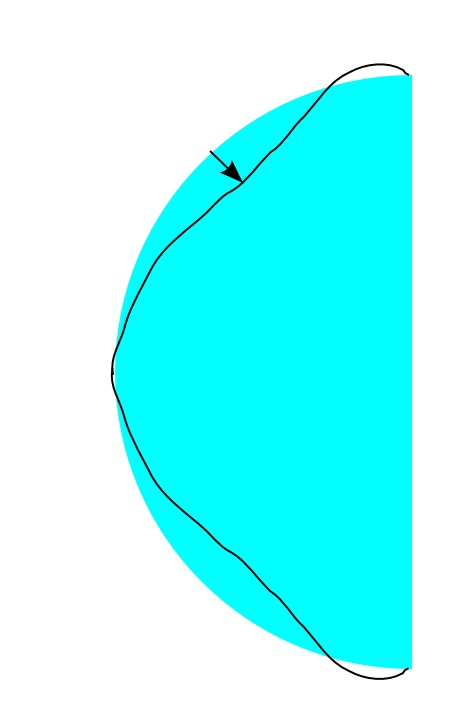
\includegraphics[width=0.3\columnwidth]{mild_asphere.jpg}\\ % added mild_asphere.svg to tree, but there is no easy way to implement this
  \caption{Sag of a mild asphere. The slope of the mild asphere terms should be orthogonal both to the slope of the sphere and the slope of each other}
  \label{fig:mild_asphere}
\end{figure}


\subsubsection{The factor $\rnorm^2 (1-\rnorm^2)$}
The polynomials tend to overshoot both at the center and at the border $\rmax$. Thus, we multiply them with a factor of zero. This ensures that the correction sag is zero both in the center and on the edge. The best-fit curvature thus determines the sag on the border.


\subsection{Introducing the Scalar Product}

The slope of the surface is more important than its position. For efficient optimization, we want a system of orthogonal functions, that are orthogonal in slope. We define the slope $S$

\begin{eqnarray}
  S_m(\rnorm) &=& \frac{\partial}{\partial \rnorm} 
	  \left(
		  \rnorm^2 (1-\rnorm^2) Q_m^{bfs}(\rnorm^2)
		\right)
\end{eqnarray}

and the scalar product

\begin{eqnarray}
  \langle Q_m^{bfs}, Q_n^{bfs} \rangle 
	&=&
	\frac{ \int_{0}^{1} d\rnorm \, S_m(\rnorm) S_n(\rnorm) \frac{1}{1 - c_{bfs} \rmax^2 \rnorm^2}  \rnorm}{ \int_{0}^{1} d\rnorm \, \frac{1}{\sqrt{1 - c_{bfs} \rmax^2 \rnorm^2}} \rnorm} \\
\end{eqnarray}

\subsection{Recursion formula}
\begin{eqnarray}
Q_0^{bfs}(\xi) &=& 1 \\
Q_1^{bfs}(\xi) &=& \frac{1}{\sqrt{19}} (13 - 16\xi) \\
Q_{m+1}^{bfs}(\xi) &=& 
  \frac{
    P^{bfs}_{m+1}(\xi) - g_m Q_{m}^{bfs}(\xi) - h_{m-1} Q_{m-1}^{bfs}(\xi) 
	}{
    f_{m+1}
	}
\end{eqnarray}
with
\begin{eqnarray}
P_0^{bfs}(\xi) &=& 2 \\
P_1^{bfs}(\xi) &=& 6 - 8\xi \\
P_{m+1}^{bfs}(\xi) &=& 
  (2-4\xi) P_{m}^{bfs}(\xi)
	-
	P_{m-1}^{bfs}(\xi)
\end{eqnarray}
and
\begin{eqnarray}
  f_0 &=& 2 \\
	f_1 &=& \frac{\sqrt{19}}{2} \\
	g_0 &=& -\frac{1}{2} \\
	h_{m-2} &=& - \frac{ m (m-1) }{2 f_{m-2}} \\
	g_{m-1} &=& - \frac{1+2g_{m-2}h_{m-2}}{f_{m-1}} \\
	f_m &=& \sqrt{ m(m+1) + 3 - g_{m-1}^2 - h_{m-2}^2 }
\end{eqnarray}

\subsection{Summary Mild Aspheres}


\section{to do: bibtex}
Shape specification for axially symmetric optical surfaces
G. W. Forbes
OPTICS EXPRESS Vol. 15, No. 8

Robust, efficient computational methods
for axially symmetric optical aspheres
G.W. Forbes
OPTICS EXPRESS Vol. 18, No. 19 

Find a better source for Jacobi Polynomials than wiki


\appendix
\section{Strong Forbes Polynomials}

\begin{eqnarray}
x &=& \r^2 / \rmax^2 \\
Q_0(x) &=& 1 \\
Q_1(x) &=& - (5 - 6x) \\
Q_2(x) &=& 15 - 14x (3 - 2x) \\
Q_3(x) &=& -(35-12x [14 - x (21-10x)]) \\
Q_4(x) &=& 70 - 3x (168- 5x[84 -11x (8 - 3x)]) \\
Q_5(x) &=& -[126 - x (1260-11x (420- x[720 -13x (45-14x)]))]
\end{eqnarray}



\end{document}